\chapter{Chimie organométallique~: liaisons et ligands}\label{ch:b3:organometallic-bonding}

En 1951, deux groupes de recherche obtinrent indépendamment une poudre
orange, stable à l'air, de formule $\ce{FeC10H10}$, qui n'avait aucun sens~:
le fer ne forme d'ordinaire pas de liaisons stables avec le carbone, et
certainement pas avec deux cycles cyclopentadiényle à la fois. En moins
d'un an, sa structure fut établie~: le fer se trouve entre deux cycles
parallèles, lié de la même façon aux dix atomes de carbone, en sandwich. Le
ferrocène a ouvert la chimie organométallique moderne, dont les catalyseurs
produisent aujourd'hui la plupart des polymères, des médicaments et des
produits de chimie fine du monde (\cref{ch:b3:homogeneous-catalysis}). Ce
chapitre explique comment les métaux se lient au monoxyde de carbone, aux
phosphines, aux alcènes, aux cycles, aux \omterm{def:b3:organometallic-bonding:carbene}{carbènes} et les uns aux autres, et
comment l'\omterm{def:b3:organometallic-bonding:isolobal}{analogie isolobale} relie les fragments organométalliques à la
chimie organique du carbone.

\begin{recall}
Le volume de première année a défini les composés organométalliques et
utilisé les réactifs de Grignard. Le volume de deuxième année a introduit la
règle des 18 électrons et le décompte des électrons de valence,
l'hapticité, les ligands $\pi$-accepteurs et $\pi$-donneurs avec la rétrodonation, les actes
élémentaires des réactions organométalliques (addition oxydante,
élimination réductrice, insertion) et les orbitales de fragments. Le
\cref{ch:b3:group-theory-applied} a dénombré les élongations CO \omterm{def:b3:group-theory-applied:activity}{actives en
IR} des carbonyles et construit des combinaisons adaptées à la symétrie~; le
\cref{ch:b3:complex-spectra-magnetism} a relié les moments magnétiques aux
électrons non appariés.
\end{recall}

\begin{omfigure}
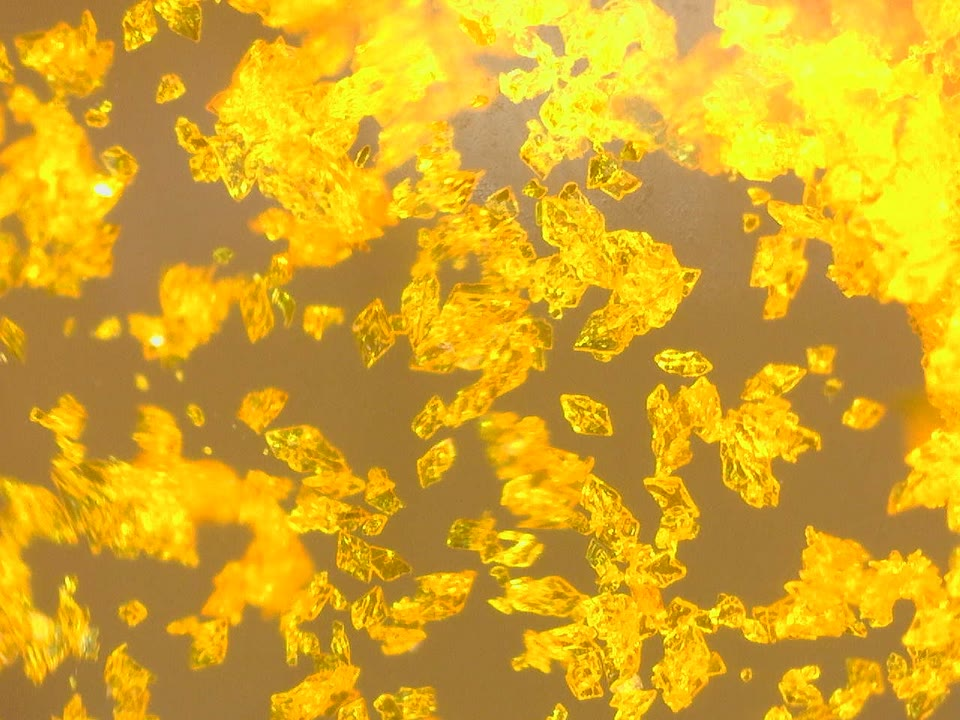
\includegraphics[width=0.5\linewidth]{images/book4/ferrocene-crystals.jpg}

{\small Cristaux de ferrocène, $\ce{Fe(C5H5)2}$~: un composé organométallique
orange, stable à l'air, qui se sublime par léger chauffage.}
\end{omfigure}

\section{Décompte des électrons et degrés d'oxydation}

\begin{method}[Compter les électrons, de deux façons]\label{met:b3:organometallic-bonding:count}
\begin{enumerate}
  \item Méthode des ligands neutres (covalente)~: le métal apporte autant
        d'électrons que son numéro de groupe~; chaque ligand, pris neutre,
        apporte 1 (H, \ce{CH3}, Cl, l'allyle
        $\eta^1$) ou 2 (CO, \ce{PR3}, alcène) ou davantage ($\eta^5$-\ce{C5H5} 5, $\eta^6$-\ce{C6H6} 6)~; ajouter un électron
        par liaison métal--métal et corriger de la charge globale.
  \item Méthode ionique~: les ligands tels que H, \ce{CH3}, Cl, \ce{C5H5}
        sont comptés comme des anions (2, 2, 2 et 6 électrons), et le métal
        comme le cation $d^n$ qui en résulte~; les ligands neutres comme
        précédemment.
  \item Les deux méthodes donnent le même total~; la méthode ionique donne
        en outre le degré d'oxydation et le nombre $d^n$.
\end{enumerate}
\end{method}

\begin{example}[Décompte]\label{ex:b3:organometallic-bonding:count}
$\ce{Fe(CO)5}$~: $8 + 5 \times 2 = 18$, fer(0), $d^8$. Ferrocène~: méthode neutre $8 + 2 \times 5 = 18$~; méthode ionique
$\ce{Fe^{2+}}$ ($d^6$, 6) $+ 2 \times 6$ ($\ce{C5H5-}$) $= 18$, fer(II). $\ce{Mn2(CO)10}$~: chaque Mn $7 + 5 \times 2 + 1$ (la liaison
Mn--Mn) $= 18$. Les complexes plans carrés $d^8$ comme $\ce{[PtCl4]^{2-}}$ ou le catalyseur de
Wilkinson $\ce{RhCl(PPh3)3}$ ont 16 électrons~: leur orbitale vide de type $p_z$ est trop
haute pour être remplie, et les complexes plans carrés à 16 électrons sont
aussi stables que les complexes à 18 électrons.
\end{example}

\section{Carbonyles et phosphines}

\begin{definition}[Carbonyles métalliques]\label{def:b3:organometallic-bonding:carbonyl}
Un \emph{carbonyle métallique}\index{carbonyle metallique@carbonyle métallique} est un complexe à ligands
monoxyde de carbone. Un \emph{carbonyle terminal}\index{carbonyle terminal}
est lié à un seul métal par le carbone~; un \emph{carbonyle pontant}\index{carbonyle pontant} relie
deux (ou trois) métaux.
\end{definition}

Ludwig Mond découvrit en 1890 que le nickel réagit avec le monoxyde de
carbone à température ordinaire pour donner le liquide volatil
$\ce{Ni(CO)4}$, qui se décompose en nickel pur par chauffage~: le principe
d'un procédé de raffinage. Le monoxyde de carbone se lie aux métaux de
transition par son orbitale la plus haute occupée, un doublet non liant
$\sigma$ situé surtout sur le carbone, et accepte des électrons dans ses
orbitales $\pi^*$ vides, elles aussi plus développées sur le carbone.

\begin{definition}[Liaison synergique]\label{def:b3:organometallic-bonding:synergic}
La \emph{liaison synergique}\index{liaison synergique} est le renforcement
mutuel de la donation $\sigma$ d'un ligand vers un métal et de la rétrodonation $\pi$ du métal
vers le ligand~: la donation enrichit le métal en électrons et le rend plus
apte à les rendre, la rétrodonation soulage la charge accumulée par la
donation.
\end{definition}

\begin{omfigure}
\begin{tikzpicture}[font=\small, >=Stealth]
  % sigma donation
  \fill[black!70] (0,0) circle (0.14); \node[anchor=north] at (0,-0.4) {M};
  \pic at (0,0) {omlobe={-0.7}{180}};
  \pic at (0,0) {omlobe={0.9}{0}};
  \node[circle, fill=black!40, inner sep=1.6pt] at (1.9,0) {};
  \node[circle, fill=omThm!70, inner sep=1.6pt] at (3.0,0) {};
  \pic at (1.9,0) {omlobe={0.85}{180}};
  \node[font=\scriptsize, anchor=north] at (1.9,-0.25) {C};
  \node[font=\scriptsize, anchor=north] at (3.0,-0.25) {O};
  \draw[->, thick, omThm] (1.4,0.55) to[bend right=30] (0.6,0.55);
  \node[anchor=north] at (1.5,-1.55) {donation $\sigma$};
  % pi back-donation
  \begin{scope}[xshift=6.0cm]
    \fill[black!70] (0,0) circle (0.14); \node[anchor=north] at (0,-1.1) {M};
    \pic at (0,0) {omdxz};
    \node[circle, fill=black!40, inner sep=1.6pt] at (1.9,0) {};
    \node[circle, fill=omThm!70, inner sep=1.6pt] at (3.0,0) {};
    \pic at (1.9,0) {omp={0.9}{90}};
    \pic at (3.0,0) {omp={-0.6}{90}};
    \draw[->, thick, omThm] (0.6,1.05) to[bend left=30] (1.6,1.05);
    \node[anchor=north] at (1.5,-1.55) {rétrodonation $\pi$};
  \end{scope}
\end{tikzpicture}

{\small \omterm{def:b3:organometallic-bonding:synergic}{Liaison synergique} du monoxyde de carbone. À gauche~: le doublet
non liant du carbone (orbitale $\sigma$) se déverse dans une orbitale vide du métal, de type
$\sigma$. À droite~: une orbitale $d$ pleine du métal ($d_{xz}$, avec ses deux axes)
recouvre l'orbitale $\pi^*$ vide de CO, plus développée sur le carbone, dont
les lobes correspondent à ses phases~: les électrons refluent dans une
orbitale antiliante entre C et O.}
\end{omfigure}

\begin{proposition}[Fréquences d'élongation de CO]\label{prop:b3:organometallic-bonding:co-frequency}
Plus un métal rétrocède d'électrons aux orbitales $\pi^*$ d'un ligand CO,
plus le nombre d'onde d'élongation C--O est bas.
\end{proposition}

\begin{proof}[Justification]
Les orbitales $\pi^*$ de CO sont antiliantes entre C et O~: les peupler
affaiblit la liaison C--O, abaisse sa \omterm{def:b3:quantum-model-systems:oscillator}{constante de force}, et donc le nombre
d'onde d'élongation, qui varie comme la racine carrée de la \omterm{def:b3:quantum-model-systems:oscillator}{constante de
force} (\cref{ch:b3:rovibrational-spectroscopy}). La donation
$\sigma$ retire des électrons d'une orbitale presque non liante (légèrement
antiliante) pour C--O, ce qui à lui seul élèverait un peu le nombre
d'onde~: la diminution observée montre que la rétrodonation domine.
\end{proof}

Le monoxyde de carbone libre a sa fondamentale à $\omega_e - 2\omega_ex_e = \qty{2143}{cm^{-1}}$~; les carbonyles
terminaux des complexes neutres absorbent à peu près entre 1900 et
\qty{2100}{cm^{-1}}, les \omterm{def:b3:organometallic-bonding:carbonyl}{carbonyles pontants} plus bas encore. Le long d'une
série isoélectronique, un carbonyle anionique absorbe à plus bas nombre
d'onde que le neutre, un carbonyle cationique plus haut~: plus le métal est
riche en électrons, plus il rétrocède. Le nombre de bandes, déduit de la
symétrie (\cref{ch:b3:group-theory-applied}), donne la géométrie.
% ledger: diat:CO.we, diat:CO.wexe

\begin{proposition}[Interactions $\pi$ et éclatement du champ des ligands]\label{prop:b3:organometallic-bonding:pi-delta}
Dans un complexe octaédrique, les ligands $\pi$-accepteurs augmentent $\Delta_{\mathrm o}$ et les ligands $\pi$-donneurs
le diminuent.
\end{proposition}

\begin{proof}
Les orbitales $e_g$ n'ont qu'une symétrie $\sigma$. Les orbitales $t_{2g}$ ($d_{xy}$, $d_{xz}$, $d_{yz}$) correspondent à une
combinaison $t_{2g}$ d'orbitales $\pi$ des ligands~: pour $d_{xy}$, les quatre ligands du plan $xy$
offrent chacun une orbitale $\pi$ perpendiculaire à leur axe M--L dans ce
plan, et la combinaison à signes alternés a la symétrie de $d_{xy}$ (les autres
combinaisons se transforment comme $t_{1g}$, $t_{1u}$ et $t_{2u}$ et ne trouvent pas de partenaire $d$). Deux orbitales de
même symétrie se mélangent et se repoussent~: la plus basse est abaissée,
la plus haute élevée. Un
accepteur $\pi$ offre des orbitales vides au-dessus du niveau $t_{2g}$, qui est abaissé~: $\Delta_{\mathrm o}$
augmente. Un donneur $\pi$ offre des orbitales pleines au-dessous de lui, qui le repoussent vers le haut~: $\Delta_{\mathrm o}$
diminue. Le niveau $e_g$ n'est affecté dans aucun des deux cas.
\end{proof}

C'est pourquoi CO et \ce{CN-} se placent à l'extrémité forte de la série
spectrochimique, et les halogénures et l'hydroxyde à l'extrémité faible,
comme l'a énoncé le volume de deuxième année.

\begin{definition}[Paramètres de Tolman]\label{def:b3:organometallic-bonding:tolman}
L'\emph{angle de cône de Tolman}\index{angle de cone de Tolman@angle de cône de Tolman} d'une phosphine est l'angle au
sommet du cône, centré sur le métal à une distance standard, qui englobe
tout juste les surfaces de van der Waals de ses substituants~: une mesure de
sa taille. Le \emph{paramètre électronique de Tolman}\index{parametre electronique de Tolman@paramètre électronique de Tolman} est le
nombre d'onde de l'élongation symétrique de CO dans $\ce{Ni(CO)3L}$~: plus la
phosphine L est donneuse, plus il est bas.
\end{definition}

Les phosphines se règlent indépendamment en taille et en pouvoir donneur
par leurs substituants~: les trialkylphosphines sont plus donneuses que les
triarylphosphines, les phosphites le sont le moins~; $\ce{P(tBu)3}$ est bien plus encombrée que $\ce{PMe3}$. Les phosphines
encombrées favorisent les faibles coordinences et la dissociation rapide
des ligands, ce qui explique leur présence dans tant de catalyseurs.

\section{Ligands $\pi$}

\begin{definition}[Modèle de Dewar--Chatt--Duncanson]\label{def:b3:organometallic-bonding:dcd}
Le \emph{modèle de Dewar--Chatt--Duncanson}\index{modele de Dewar--Chatt--Duncanson@modèle de Dewar--Chatt--Duncanson} de la
liaison d'un alcène à un métal combine la donation $\sigma$ de l'orbitale $\pi$ de C=C
vers une orbitale vide du métal et la rétrodonation d'une orbitale $d$
pleine du métal vers l'orbitale $\pi^*$ de C=C. Sa limite de forte
rétrodonation est un \emph{métallacyclopropane}\index{metallacyclopropane@métallacyclopropane}, un cycle à
trois chaînons avec deux liaisons $\sigma$ M--C et une liaison simple C--C.
\end{definition}

\begin{proposition}[Conséquences de la rétrodonation vers un alcène]\label{prop:b3:organometallic-bonding:dcd}
La coordination allonge la liaison C=C et rabat les substituants en arrière,
à l'opposé du métal, d'autant plus que la rétrodonation augmente.
\end{proposition}

\begin{proof}[Justification]
Retirer des électrons de l'orbitale $\pi$ (liante) et en ajouter dans
l'orbitale $\pi^*$ (antiliante) abaissent tous deux l'indice de liaison C--C.
Le mélange avec $\pi^*$ réhybride les carbones vers $sp^3$, dont les
liaisons aux substituants pointent à l'opposé du métal, vers la géométrie
du \omterm{def:b3:organometallic-bonding:dcd}{métallacyclopropane}.
\end{proof}

\begin{omfigure}
\begin{tikzpicture}[font=\small, >=Stealth]
  \fill[black!70] (0,0) circle (0.14); \node[anchor=north] at (0,-1.1) {M};
  \pic at (0,0) {omlobe={0.9}{0}};
  \foreach \y in {0.45,-0.45}{\node[circle, fill=black!40, inner sep=1.6pt] at (1.9,\y) {};}
  \pic at (1.9,0.45) {omp={-0.75}{0}};
  \pic at (1.9,-0.45) {omp={-0.75}{0}};
  \draw[->, thick, omThm] (1.3,1.0) to[bend right=30] (0.5,0.6);
  \node[anchor=north] at (1.2,-1.4) {$\sigma$~: $\pi$(C=C) $\to$ M};
  \begin{scope}[xshift=5.6cm]
    \fill[black!70] (0,0) circle (0.14); \node[anchor=north] at (0,-1.1) {M};
    \pic at (0,0) {omdxy};
    \foreach \y in {0.45,-0.45}{\node[circle, fill=black!40, inner sep=1.6pt] at (1.9,\y) {};}
    \pic at (1.9,0.45) {omp={-0.75}{0}};
    \pic at (1.9,-0.45) {omp={0.75}{0}};
    \draw[->, thick, omThm] (0.7,0.9) to[bend left=30] (1.5,0.9);
    \node[anchor=north] at (1.2,-1.4) {$\pi$~: M $\to$ $\pi^*$(C=C)};
  \end{scope}
\end{tikzpicture}

{\small Le \omterm{def:b3:organometallic-bonding:dcd}{modèle de Dewar--Chatt--Duncanson} d'un alcène lié par le côté
(C=C vertical, le métal à gauche). À gauche~: l'orbitale $\pi$ pleine (deux orbitales $p$
en phase) se déverse dans une orbitale vide du métal. À droite~: une
orbitale $d$ pleine du métal, de phases appropriées, se déverse dans l'orbitale $\pi^*$
vide (les deux orbitales $p$ en opposition de phase).}
\end{omfigure}

Le sel de Zeise, $\ce{K[PtCl3(C2H4)]}$, préparé en 1827, fut le premier composé
organométallique d'un métal de transition~; son éthène est perpendiculaire
au plan \ce{PtCl3}, comme le prévoit le modèle. L'allyle ($\eta^3$), les diènes ($\eta^4$), les arènes ($\eta^6$) et le cycle
cyclopentadiényle ($\eta^5$) se lient de la même façon, par plusieurs
carbones à la fois.

\begin{definition}[Métallocènes]\label{def:b3:organometallic-bonding:metallocene}
Un \emph{composé sandwich}\index{compose sandwich@composé sandwich} possède un métal entre deux
ligands cycliques plans et parallèles, liés par tous leurs carbones~; un
\emph{métallocène}\index{metallocene@métallocène} est un composé sandwich à deux cycles $\eta^5$-cyclopentadiényle,
$\ce{M(C5H5)2}$.
\end{definition}

\begin{proposition}[Les orbitales frontières du ferrocène]\label{prop:b3:organometallic-bonding:ferrocene}
Dans un \omterm{def:b3:organometallic-bonding:metallocene}{métallocène} à cycles parallèles ($D_{5d}$), les orbitales $d$ du métal se scindent en $e_{2g}$
($d_{xy}$, $d_{x^2-y^2}$) et $a_{1g}$ ($d_{z^2}$), presque non liantes et proches l'une de l'autre, et $e_{1g}^\ast$ ($d_{xz}$,
$d_{yz}$), fortement antiliantes~; le ferrocène, avec six électrons $d$ en $e_{2g}^4a_{1g}^2$, a 18
électrons et aucun électron non apparié.
\end{proposition}

\begin{proof}[Justification]
Les orbitales $\pi$ des deux cycles se combinent en paires adaptées à la symétrie $a_{1g}$, $a_{2u}$,
$e_{1g}$, $e_{1u}$, $e_{2g}$, $e_{2u}$ (à partir des cinq orbitales $\pi$ de chaque cycle, avec zéro, un et deux
plans nodaux contenant l'axe). La combinaison $e_{1g}$ pleine des cycles
recouvre fortement $d_{xz}$, $d_{yz}$ (un plan nodal contenant l'axe chacune)~: elles forment des orbitales
liantes, surtout centrées sur les cycles, et des antiliantes $e_{1g}^\ast$, surtout centrées sur le métal, rejetées vers le haut. $d_{xy}$, $d_{x^2-y^2}$
(deux plans nodaux) ne rencontrent que les orbitales $e_{2g}$ vides des cycles
et sont légèrement stabilisées par rétrodonation~; $d_{z^2}$ pointe vers le trou au centre de chaque cycle et
ne recouvre presque rien. Six électrons remplissent $e_{2g}$ et $a_{1g}$~; avec les douze électrons des
combinaisons liantes des cycles, le décompte est de 18.
\end{proof}

\begin{omfigure}
\begin{tikzpicture}[font=\small]
  % sandwich drawing
  \begin{scope}[xshift=-1.0cm]
    \draw[thick, fill=black!8] (0,1.0) ellipse (1.0 and 0.3);
    \draw[thick, fill=black!8] (0,-1.0) ellipse (1.0 and 0.3);
    \foreach \a in {90,162,234,306,18}{\fill[black!60] ({cos(\a)},{1.0+0.3*sin(\a)}) circle (0.07);
      \fill[black!60] ({cos(\a)},{-1.0+0.3*sin(\a)}) circle (0.07);}
    \shade[ball color=orange!70!brown] (0,0) circle (0.2);
    \node[anchor=west] at (0.25,0) {Fe};
  \end{scope}
  % diagramme de niveaux de quatre métallocènes
  \pic[transform shape] at (2.1,-0.9) {omlevel={u}{0.5}};
  \pic[transform shape] at (2.7,-0.9) {omlevel={ud}{0.5}};
  \pic[transform shape] at (2.4,-0.4) {omlevel={ud}{0.5}};
  \pic[transform shape] at (2.1,1.0) {omlevel={}{0.5}};
  \pic[transform shape] at (2.7,1.0) {omlevel={}{0.5}};
  \node[anchor=north] at (2.4,-1.3) {\ce{[FeCp2]+}};
  \node[anchor=north, font=\scriptsize] at (2.4,-1.75) {17 e$^-$};
  \pic[transform shape] at (4.3,-0.9) {omlevel={ud}{0.5}};
  \pic[transform shape] at (4.9,-0.9) {omlevel={ud}{0.5}};
  \pic[transform shape] at (4.6,-0.4) {omlevel={ud}{0.5}};
  \pic[transform shape] at (4.3,1.0) {omlevel={}{0.5}};
  \pic[transform shape] at (4.9,1.0) {omlevel={}{0.5}};
  \node[anchor=north] at (4.6,-1.3) {\ce{FeCp2}};
  \node[anchor=north, font=\scriptsize] at (4.6,-1.75) {18 e$^-$};
  \pic[transform shape] at (6.5,-0.9) {omlevel={ud}{0.5}};
  \pic[transform shape] at (7.1,-0.9) {omlevel={ud}{0.5}};
  \pic[transform shape] at (6.8,-0.4) {omlevel={ud}{0.5}};
  \pic[transform shape] at (6.5,1.0) {omlevel={u}{0.5}};
  \pic[transform shape] at (7.1,1.0) {omlevel={}{0.5}};
  \node[anchor=north] at (6.8,-1.3) {\ce{CoCp2}};
  \node[anchor=north, font=\scriptsize] at (6.8,-1.75) {19 e$^-$};
  \pic[transform shape] at (8.7,-0.9) {omlevel={ud}{0.5}};
  \pic[transform shape] at (9.3,-0.9) {omlevel={ud}{0.5}};
  \pic[transform shape] at (9.0,-0.4) {omlevel={ud}{0.5}};
  \pic[transform shape] at (8.7,1.0) {omlevel={u}{0.5}};
  \pic[transform shape] at (9.3,1.0) {omlevel={u}{0.5}};
  \node[anchor=north] at (9.0,-1.3) {\ce{NiCp2}};
  \node[anchor=north, font=\scriptsize] at (9.0,-1.75) {20 e$^-$};
  \node[anchor=east, font=\scriptsize] at (1.8,-0.9) {$e_{2g}$};
  \node[anchor=east, font=\scriptsize] at (1.8,-0.4) {$a_{1g}$};
  \node[anchor=east, font=\scriptsize] at (1.8,1.0) {$e_{1g}^\ast$};
\end{tikzpicture}

{\small À gauche~: la structure sandwich du ferrocène (cycles éclipsés). À
droite~: les orbitales frontières à dominante $d$ des \omterm{def:b3:organometallic-bonding:metallocene}{métallocènes}, $e_{2g}$ et $a_{1g}$ presque non liantes, $e_{1g}^\ast$
antiliantes, remplies pour le cation ferrocénium (17 électrons), le
ferrocène (18), le cobaltocène (19) et le nickelocène (20, un électron dans
chaque orbitale $e_{1g}^\ast$, spins parallèles selon la règle de Hund).}
\end{omfigure}

\section{Carbènes, carbynes et liaisons métal--métal}

\begin{definition}[Carbènes et complexes carbéniques]\label{def:b3:organometallic-bonding:carbene}
Un \emph{carbène}\index{carbene@carbène} est une espèce neutre $\ce{R2C}$ comportant un carbone
divalent porteur de deux électrons non liants. Un \emph{complexe carbénique}\index{complexe carbenique@complexe carbénique}
possède un ligand $\ce{CR2}$ lié à un métal par une double liaison, $\ce{M=CR2}$. Un complexe
de \emph{carbène de Fischer}\index{carbene de Fischer@carbène de Fischer} porte un substituant hétéroatomique sur le
carbone carbénique et un métal à bas degré d'oxydation entouré de ligands $\pi$-accepteurs~; son carbone
carbénique est électrophile. Un complexe de \emph{carbène de Schrock}\index{carbene de Schrock@carbène de Schrock}
(alkylidène) ne porte que des substituants C ou H et un métal de début de
série à haut degré d'oxydation~; son carbone est nucléophile. Un \emph{carbène N-hétérocyclique}\index{carbene N-heterocyclique@carbène N-hétérocyclique} est un
carbène cyclique encadré par deux atomes d'azote, stable à l'état libre et
ligand fortement donneur
$\sigma$.
\end{definition}

Les deux sortes de \omterm{def:b3:organometallic-bonding:carbene}{complexes carbéniques} diffèrent par la façon dont la
liaison M=C est partagée. Dans un \omterm{def:b3:organometallic-bonding:carbene}{carbène de Fischer}, un \omterm{def:b3:organometallic-bonding:carbene}{carbène} singulet
donne son doublet au métal et reçoit en retour une rétrodonation dans son
orbitale $p$ vide, que le doublet de l'hétéroatome stabilise aussi~: le
carbone reste pauvre en électrons et subit l'attaque des nucléophiles. Dans
un \omterm{def:b3:organometallic-bonding:carbene}{carbène de Schrock}, deux fragments triplets, le métal et le \omterm{def:b3:organometallic-bonding:carbene}{carbène},
forment une liaison covalente $\sigma +
\pi$, polarisée vers le carbone~: l'alkylidène se comporte comme un ylure de Wittig.

\begin{definition}[Complexe carbynique]\label{def:b3:organometallic-bonding:carbyne}
Un \emph{complexe carbynique}\index{complexe carbynique} possède une triple
liaison entre un métal et un carbone porteur d'un seul substituant, $\ce{M#CR}$.
\end{definition}

\begin{definition}[Liaison $\delta$, liaison quadruple]\label{def:b3:organometallic-bonding:delta}
Une \emph{liaison $\delta$}\index{liaison delta@liaison $\delta$} est une liaison dont l'orbitale possède deux plans nodaux
contenant l'axe internucléaire, formée par le recouvrement face à face de
deux orbitales $d$ telles que $d_{xy}$ et $d_{xy}$. Une \emph{liaison quadruple}\index{liaison quadruple}
combine une liaison $\sigma$, deux liaisons $\pi$ et une liaison $\delta$ entre deux atomes métalliques.
\end{definition}

\begin{proposition}[{La \omterm{def:b3:organometallic-bonding:delta}{liaison quadruple} de $[\mathrm{Re_2Cl_8}]^{2-}$}]\label{prop:b3:organometallic-bonding:quadruple}
Dans $\ce{[Re2Cl8]^{2-}}$ (deux \ce{Re^{III}}, $d^4$ chacun), les huit électrons $d$ occupent $\sigma^2\pi^4\delta^2$~: un
indice de liaison de 4, qui impose la disposition éclipsée des deux unités
\ce{ReCl4}.
\end{proposition}

\begin{proof}
Avec $z$ selon l'axe Re--Re et les atomes Cl selon $\pm x$ et $\pm y$ sur chaque Re, $d_{x^2-y^2}$
pointe vers les chlorures et sert aux liaisons Re--Cl. Les quatre autres orbitales $d$
de chaque métal se recouvrent deux à deux~: $d_{z^2}$ avec $d_{z^2}$ le long de l'axe ($\sigma$), $d_{xz}$ avec $d_{xz}$ et $d_{yz}$
avec $d_{yz}$ côte à côte ($\pi$, deux fois), $d_{xy}$ avec $d_{xy}$ face à face ($\delta$, la plus faible).
Huit électrons remplissent les quatre combinaisons liantes. Tourner une
unité de $45^\circ$ autour de $z$ change son $d_{xy}$ en $d_{x^2-y^2}$, dont le recouvrement avec l'autre $d_{xy}$ est
nul par symétrie~: la liaison $\delta$, et avec elle la préférence pour la
conformation éclipsée, est perdue. Les trois autres recouvrements sont de
symétrie cylindrique ou inchangés en valeur absolue.
\end{proof}

% ledger: geom:Re2Cl8.ReRe
La distance Re--Re de \qty{2.24}{\angstrom} dans le sel de potassium est très courte pour deux atomes métalliques, et les chlorures des deux moitiés sont bel et bien éclipsés, malgré
leur répulsion stérique~: la liaison $\delta$, si faible soit-elle, les maintient ainsi.

\begin{omfigure}
\tdplotsetmaincoords{58}{25}
\begin{tikzpicture}[tdplot_main_coords, font=\small, scale=1.15]
  \draw[thick, black!60] (0,0,0) -- (0,0,2.0);
  \foreach \z in {0,2.0}{
    \foreach \b in {0,90,180,270}{
      \draw[black!45] (0,0,\z) -- ({1.55*cos(\b)},{1.55*sin(\b)},\z);}
    \foreach \a/\s in {45/omphasepos, 135/omphaseneg, 225/omphasepos, 315/omphaseneg}{
      \path[\s, opacity=0.9] plot[domain=0:360, samples=48, smooth cycle]
        ({0.62*cos(\a)+0.55*cos(\x)*cos(\a)-0.26*sin(\x)*sin(\a)},
         {0.62*sin(\a)+0.55*cos(\x)*sin(\a)+0.26*sin(\x)*cos(\a)}, {\z});}
    \foreach \b in {0,90,180,270}{
      \node[circle, fill=green!45!black, inner sep=1.8pt] at ({1.55*cos(\b)},{1.55*sin(\b)},\z) {};}
    \shade[ball color=black!40] (0,0,\z) circle (0.14);}
  \node[anchor=east, xshift=-1.9cm] at (0,0,2.0) {Re};
  \node[anchor=east, xshift=-1.9cm] at (0,0,0) {Re};
\end{tikzpicture}

{\small La composante $\delta$ de la \omterm{def:b3:organometallic-bonding:delta}{liaison quadruple} de $\ce{[Re2Cl8]^{2-}}$~: les orbitales $d_{xy}$ des
deux atomes de rhénium (quatre lobes chacune, signes en bleu et en orange)
se font face de part et d'autre de l'axe Re--Re, lobe contre lobe de même
signe. Les chlorures (en vert), éclipsés, se trouvent selon $x$ et $y$, entre les lobes.}
\end{omfigure}

\section{L'analogie isolobale}

\begin{definition}[Fragments isolobaux]\label{def:b3:organometallic-bonding:isolobal}
Deux fragments moléculaires sont \emph{isolobaux}\index{fragments isolobaux}
lorsque le nombre, la symétrie, l'énergie approximative et la forme de leurs
orbitales frontières, ainsi que le nombre d'électrons qu'elles contiennent,
sont semblables. L'\emph{analogie isolobale}\index{analogie isolobale} prévoit
que des fragments isolobaux peuvent se remplacer l'un l'autre dans les
molécules.
\end{definition}

\begin{proposition}[Séries isolobales]\label{prop:b3:organometallic-bonding:isolobal}
$\ce{CH3}$, $\ce{Mn(CO)5}$ et $\ce{CpFe(CO)2}$ sont \omterm{def:b3:organometallic-bonding:isolobal}{isolobaux} (une orbitale frontière, un électron)~;
$\ce{CH2}$ et $\ce{Fe(CO)4}$ (deux orbitales, deux électrons)~; $\ce{CH}$ et $\ce{Co(CO)3}$ (trois orbitales,
trois électrons).
\end{proposition}

\begin{proof}[Justification]
$\ce{CH3}$ est un fragment tétraédrique auquel il manque une liaison~: une orbitale de type $sp^3$ avec un
électron, un de moins que l'octet. $\ce{Mn(CO)5}$ est un octaèdre auquel il manque un ligand~: le
site vacant porte une orbitale hybride pointée vers l'extérieur~; avec $7 + 10 = 17$ électrons, il lui en manque
un pour atteindre 18, et son électron célibataire occupe cet hybride.
Retirer deux ou trois ligands (ou liaisons) donne deux ou trois orbitales
et électrons de ce type, avec le même décompte des deux côtés~: $\ce{Fe(CO)4}$ a 16 électrons ($8 + 8$), deux de moins que 18~;
$\ce{Co(CO)3}$ en a 15 ($9 + 6$), trois de moins.
\end{proof}

\begin{method}[Prévoir une structure par remplacement isolobal]\label{met:b3:organometallic-bonding:isolobal}
\begin{enumerate}
  \item Découper le composé en fragments et compter pour chacun les
        orbitales frontières et les électrons.
  \item Remplacer chaque fragment par son partenaire organique isolobal.
  \item L'analogue organique, s'il existe, suggère la liaison et la forme~:
        $\ce{Mn2(CO)10}$ est un «~éthane~», $\ce{Co3(CO)9CH}$ est un «~tétraédrane~» $\ce{(CH)4}$ dont trois CH
        sont remplacés par $\ce{Co(CO)3}$.
\end{enumerate}
\end{method}

\begin{omfigure}
\begin{tikzpicture}[font=\small]
  \foreach \y/\l/\r/\n in {0/{\ce{CH3}}/{\ce{Mn(CO)5}}/1, -1.6/{\ce{CH2}}/{\ce{Fe(CO)4}}/2, -3.2/{\ce{CH}}/{\ce{Co(CO)3}}/3}{
    \node at (0,\y) {\l};
    \node at (5.2,\y) {\r};
    \node[font=\large] at (2.6,\y) {$\longleftrightarrow$};
    \node[font=\scriptsize, anchor=south] at (2.6,\y+0.15) {isolobaux};
    \node[font=\scriptsize, anchor=west] at (7.0,\y) {\ifnum\n=1 une orbitale frontière, un électron\else\ifnum\n=2 deux orbitales frontières, deux électrons\else trois orbitales frontières, trois électrons\fi\fi};}
  \foreach \a in {0}{\pic at (0.55,0) {omlobe={0.6}{0}};}
  \pic at (6.25,0) {omlobe={0.6}{0}};
  \pic at (0.45,-1.6) {omlobe={0.6}{20}}; \pic at (0.45,-1.6) {omlobe={0.6}{-20}};
  \pic at (6.15,-1.6) {omlobe={0.6}{20}}; \pic at (6.15,-1.6) {omlobe={0.6}{-20}};
  \foreach \t in {-30,0,30}{\pic at (0.4,-3.2) {omlobe={0.55}{\t}}; \pic at (6.1,-3.2) {omlobe={0.55}{\t}};}
\end{tikzpicture}

{\small Les séries isolobales (hybrides frontières dessinés
schématiquement)~: chaque fragment organique et le fragment \omterm{def:b3:organometallic-bonding:carbonyl}{carbonyle
métallique} qui lui fait face ont le même nombre d'orbitales frontières
pointées vers l'extérieur et d'électrons dans ces orbitales, et se combinent
de façon analogue.}
\end{omfigure}

\begin{definition}[Interaction agostique]\label{def:b3:organometallic-bonding:agostic}
Une \emph{interaction agostique}\index{interaction agostique} est une liaison
à trois centres et deux électrons entre un métal et une liaison C--H de l'un
de ses propres ligands, dans laquelle le doublet liant C--H se déverse dans
une orbitale vide du métal.
\end{definition}

Les hydrogènes agostiques se manifestent par des distances métal--hydrogène
courtes dans les structures de diffraction, par des nombres d'onde
d'élongation C--H anormalement bas et, en RMN, par un déplacement vers les
champs forts et un couplage $^1J_{\mathrm{CH}}$ réduit. Ce sont des instantanés figés de
l'activation C--H, première étape de nombreuses réactions catalytiques.

\begin{inthelab}[Travailler avec des carbonyles métalliques]
Les \omterm{def:b3:organometallic-bonding:carbonyl}{carbonyles métalliques} se manipulent sous une hotte dont l'extraction
fonctionne, sous diazote ou argon, sans flamme nue~: beaucoup libèrent du
monoxyde de carbone quand on les chauffe. Les carbonyles volatils se
transfèrent par canule ou sur une rampe à vide, jamais par simple
versement~; les résidus sont détruits par oxydation lente (eau de Javel ou
eau de brome) sous la hotte. Le nickel tétracarbonyle, le plus dangereux,
n'est pas du tout utilisé dans les laboratoires d'enseignement.
\end{inthelab}

\begin{safety}{\ghs[0.62cm]{GHS02}\ghs[0.62cm]{GHS06}\ghs[0.62cm]{GHS07}\ghs[0.62cm]{GHS08}\ghs[0.62cm]{GHS09}}
% ledger: ghs4:NiCO4, ghs4:ferrocene
Nickel tétracarbonyle~: extrêmement inflammable, mortel par inhalation,
susceptible de provoquer le cancer, peut nuire au fœtus. Ferrocène~: solide
inflammable, nocif en cas d'ingestion~; manipulé comme un produit de chimie
fine, avec des gants et des précautions contre les poussières.
\end{safety}

\begin{history}[Le carbonyle de Mond et le sandwich]
Ludwig Mond et ses collaborateurs découvrirent le nickel tétracarbonyle en
1890 en étudiant la corrosion de vannes en nickel par le monoxyde de
carbone, et fondèrent sur lui un procédé de raffinage du nickel. Le
ferrocène fut préparé en 1951 par Thomas Kealy et Peter Pauson, et
indépendamment par Samuel Miller, John Tebboth et John Tremaine~; en 1952,
Geoffrey Wilkinson et Robert Woodward, ainsi qu'Ernst Otto Fischer,
proposèrent la structure sandwich. Fischer et Wilkinson partagèrent le prix
Nobel de chimie 1973 pour leurs travaux sur les \omterm{def:b3:organometallic-bonding:metallocene}{composés sandwichs}.
\end{history}

\section{Exercices}

\begin{exercise}[$\star$]\label{exo:b3:organometallic-bonding:1}
Compter les électrons de valence de $\ce{Fe(CO)5}$, $\ce{Mn2(CO)10}$ (par Mn), $\ce{CpMo(CO)3H}$, de l'anion de Zeise
$\ce{[PtCl3(C2H4)]-}$, de $\ce{Cr($\eta^6$-C6H6)(CO)3}$ et de $\ce{Cp2ZrCl2}$.
\end{exercise}

\begin{exercise}[$\star$]\label{exo:b3:organometallic-bonding:2}
Donner le degré d'oxydation et le nombre $d^n$ du métal dans chaque composé
de l'exercice précédent.
\end{exercise}

\begin{exercise}[$\star$]\label{exo:b3:organometallic-bonding:3}
Classer les nombres d'onde d'élongation de CO de $\ce{[V(CO)6]-}$, $\ce{Cr(CO)6}$ et $\ce{[Mn(CO)6]+}$, en justifiant.
\end{exercise}

\begin{exercise}[$\star$]\label{exo:b3:organometallic-bonding:4}
Donner les analogues organiques \omterm{def:b3:organometallic-bonding:isolobal}{isolobaux} de $\ce{Mn2(CO)10}$, $\ce{[CpFe(CO)2]2}$ et $\ce{Co3(CO)9CH}$.
\end{exercise}

\begin{exercise}[$\star\star$]\label{exo:b3:organometallic-bonding:5}
Combien de bandes d'élongation de CO les isomères $fac$- et $mer$-$\ce{M(CO)3L3}$ présentent-ils en IR~?
\end{exercise}

\begin{exercise}[$\star\star$]\label{exo:b3:organometallic-bonding:6}
Expliquer pourquoi remplacer $\ce{PMe3}$ par $\ce{P(tBu)3}$ dans un catalyseur peut accélérer une étape qui exige
qu'un ligand quitte le métal.
\end{exercise}

\begin{exercise}[$\star\star$]\label{exo:b3:organometallic-bonding:7}
Classer $\ce{(CO)5Cr=C(OMe)Ph}$ et $\ce{Ta(=CHCMe3)(CH2CMe3)3}$ parmi les complexes de \omterm{def:b3:organometallic-bonding:carbene}{carbène de
Fischer} ou de Schrock, et prévoir leurs réactions avec une amine et avec une
cétone.
\end{exercise}

\begin{exercise}[$\star\star$]\label{exo:b3:organometallic-bonding:8}
Quel indice de liaison aurait un $\ce{[Re2Cl8]^{2-}}$ décalé~? Quel est l'indice de liaison de
$\ce{[Re2Cl8]^{4-}}$, qui a deux électrons de plus~?
\end{exercise}

\begin{exercise}[$\star\star$]\label{exo:b3:organometallic-bonding:9}
Citer trois types d'indices d'une interaction C--H agostique.
\end{exercise}

\begin{exercise}[$\star\star\star$]\label{exo:b3:organometallic-bonding:10}
Donner des exemples de complexes stables à 16, 17 et 19 électrons de
valence, et expliquer chaque exception à la règle des 18 électrons.
\end{exercise}

\begin{exercise}[$\star\star\star$]\label{exo:b3:organometallic-bonding:11}
$\ce{Cr(CO)6}$ est incolore et diamagnétique. Expliquer, à l'aide de l'effet $\pi$-accepteur sur $\Delta_{\mathrm o}$,
pourquoi il est bas spin et pourquoi ses bandes $d$--$d$ se situent dans l'ultraviolet.
\end{exercise}

\begin{exercise}[$\star\star\star$]\label{exo:b3:organometallic-bonding:12}
La liaison C--C de l'éthène s'allonge de \qty{1.34}{\angstrom} à
\qty{1.37}{\angstrom} dans le sel de Zeise et jusqu'à environ
\qty{1.43}{\angstrom} dans un complexe d'un métal à bas degré d'oxydation
avec une forte rétrodonation (données de l'exercice). Interpréter à l'aide
du \omterm{def:b3:organometallic-bonding:dcd}{modèle de Dewar--Chatt--Duncanson}.
\end{exercise}

\section{Problème~: des sandwichs}

\begin{problem}[{Problème du week-end --- des sandwichs~: décompte des
électrons de quatre métallocènes, leurs orbitales frontières et leurs
électrons non appariés, leur chimie redox, et deux questions sur les
fragments isolobaux et la spectroscopie}]
\label{pb:b3:organometallic-bonding:1}
Les \omterm{def:b3:organometallic-bonding:metallocene}{métallocènes} $\ce{MCp2}$ ($\ce{Cp} = \eta^5$-$\ce{C5H5}$) sont connus pour M = Fe, Co, Ni et pour le cation ferrocénium.

\medskip\noindent\textbf{Partie I --- Décompte.}
\begin{enumerate}
  \item Compter les électrons du ferrocène par la méthode ionique.
  \item Les compter par la méthode neutre.
  \item Faire le décompte du cobaltocène.
  \item Faire le décompte du nickelocène.
  \item Faire le décompte du cation ferrocénium.
  \item Donner le degré d'oxydation et le nombre $d^n$ de chaque métal.
\end{enumerate}

\medskip\noindent\textbf{Partie II --- Orbitales et magnétisme.}
\begin{enumerate}[resume]
  \item Classer les cinq orbitales $d$ dans $D_{5d}$.
  \item Lesquelles recouvrent fortement les orbitales $\pi$ des cycles, et
        avec quelle conséquence~?
  \item Donner l'ordre des niveaux à dominante $d$.
  \item Les remplir pour le ferrocène~: électrons non appariés~?
  \item Les remplir pour le cobaltocène~: électrons non appariés et \omterm{def:b3:complex-spectra-magnetism:moment}{moment
        de spin seul}~?
  \item Les remplir pour le nickelocène~: électrons non appariés et \omterm{def:b3:complex-spectra-magnetism:moment}{moment
        de spin seul}~?
  \item Les remplir pour le ferrocénium~: électrons non appariés~? Pourquoi
        son moment mesuré dépasse-t-il la valeur de spin seul~?
\end{enumerate}

\medskip\noindent\textbf{Partie III --- Oxydoréduction.}
\begin{enumerate}[resume]
  \item Pourquoi le cobaltocène est-il un réducteur fort~?
  \item Pourquoi le couple ferrocène/ferrocénium est-il rapide et
        réversible~?
  \item Pourquoi l'utilise-t-on comme référence interne en électrochimie
        non aqueuse (\cref{ch:b3:electrode-kinetics})~?
  \item Qu'attendre des réactions du nickelocène avec des ligands à deux
        électrons~?
\end{enumerate}

\medskip\noindent\textbf{Partie IV --- Fragments et spectres.}
\begin{enumerate}[resume]
  \item Montrer que $\ce{CpFe(CO)2}$ est isolobal à \ce{CH3}, et prévoir la structure de
        $\ce{[CpFe(CO)2]2}$.
  \item Quel dimère mixte pourrait-il former avec $\ce{Mn(CO)5}$~?
  \item Comment le remplacement d'un CO de $\ce{CpMn(CO)3}$ par $\ce{PPh3}$ modifie-t-il les
        élongations des CO restants~?
  \item Combien de bandes de CO présente $\ce{Cr($\eta^6$-C6H6)(CO)3}$ ($C_{3v}$)~?
  \item Pourquoi un cycle Cp $\eta^5$ peut-il glisser vers $\eta^3$ au cours d'une substitution~?
  \item Énoncer le résultat~: le moment magnétique de spin seul du
        nickelocène.
\end{enumerate}
\end{problem}
